\documentclass[article,a4paper]{IEEEtran}
\usepackage{lipsum}
\usepackage[backend=biber]{biblatex}
\usepackage{graphicx}

\addbibresource{refs.bib}
\title{IIoT's need for edge computing with AI capabilities for more securely transformation into industry 4.0}
\author{
\IEEEauthorblockN{Anton Odén}\\
\IEEEauthorblockA{Dept. of Maths and Computer Science\\Karlstad University\\
651 88 KARLSTAD, Sweden}\\
anton.oden@outlook.com
}

\begin{document}

\maketitle

\begin{abstract}
    The expansion of Industrial IoT (IIoT) introduces significant cybersecurity challenges, including botnet attacks, identity spoofing, and ransomware threats. AI-driven security solutions and edge computing play a role in mitigating these risks by enabling real-time threat detection and decentralized identity management. While leveraging edge computing, factory plants minimize latency while strengthen their in-house technical capabilities, fostering innovation and resilience.
\end{abstract}

\tableofcontents

\section{Introduction}
The grooving interconnectivity between devices, sensors and cloud systems exposes industrial networks to various cyber security threats. Industry 4.0's goal with IoT to connect all things create such great mass of data and datapoints that is being impossible by human to handle without advanced security algorithms. This article is based upon two recent articles providing insights into how technologies within big data analytics, deep learning and edge computing can strengthen IIoT security. Discussing confidentiality, integrity, authentication, access control etc.     
\newline\newline
The first paper \cite{SurveySecurity}, a "A Survey on Industrial Internet of Things Security: Requirements, Attacks, AI-Based Solutions, and Edge Computing Opportunities" by Bandar Alotaibi discuss key security challenges in IIoT ecosystems, highlighting vulnerabilities across perception (end nodes), network and application layer. It is rich in examples being a survey of many papers and promotes implementing intrusion detection systems in edge computing locations for easier findings and blocking of maliouses software.   
\newline\newline
Second paper \cite{Deeplearning} "Internet of Things Security Based on Big Data and Deep Learning" by Jian-Liang Wang and Ping Chen, focuses on how deep learning techniques can enhance IoT security. 

Both papers illustrate how AI-powered solutions can create more resilient industrial networks. This article examine their findings and explore how industries can integrate big-data driven security to safeguard IIoT systems.
\begin{figure}
    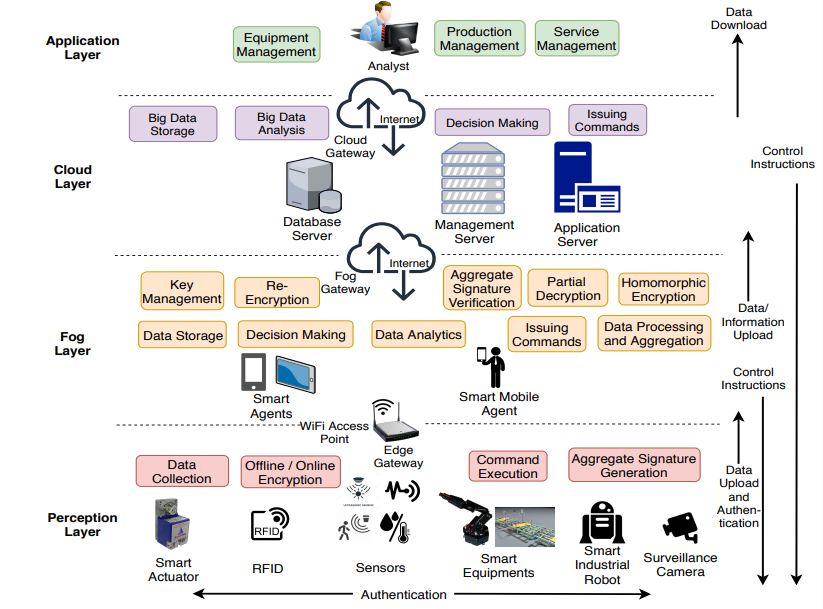
\includegraphics[width=\columnwidth]{Fog-basedarchitecture.png}
    \caption{ Proposed edge/fog architecture from \cite{fog} }
    \label{fig3: Architecture }
\end{figure}
\section{Security Challenges in Industrial IoT}
As industries continue to implement IoT technologies the digital transformation also exposes vulnerabilities, making security a priority within Industrial IoT (IIoT). Unlike traditional IT infrastructure, IIoT environments consist of distributed devices of which many operates in remote industrial locations. This decentralization creates a wide attack surface being more difficult to monitor and defend against threats. 
\newline\newline
Many industrial machinery also rely on outdated hardware and software, originally designed with less or no modern cybersecurity considerations. These systems often lack encryption, secure authentication and patching protocols, making them easy targets \cite{SurveySecurity}. Additionally, the absence of universal security standards complicates efforts to implement consistent protection across different IIoT deployments. Security breaches aren't all coming directly from external sources either. Insider threats, whether intentional or accidental pose a big risk to IIoT systems. Weak access controls, improper credential management, and lack of employee cybersecurity awareness can lead to unauthorized access, data leaks, system failures, ransomware etc. 
\newline\newline
IIoT networks are also reliant or often integrate components from multiple vendors, introducing risks related to third-party software vulnerabilities and potential backdoor access \cite{fog}. If a supplier experiences a security breach, attacker could use compromised information about that vendors devices to infiltrate industrial infrastructure.
\section{Types of Cyberattacks Threatening IIoT Systems}
Attackers exploit vulnerabilities across different layers of IIoT architecture, potentially causing operational disruption, financial losses, safety hazards and more. This section explores the most prominent cyberattacks targeting IIoT systems. 
\subsection{Perception Layer Attacks}
The perception layer consists of various objects, such as sensors, cameras, robots and smart meters. This layer is responsible of gathering data/information, for example vibrations, heat, acceleration, or humidity. The collected data is then transmitted in the network layer to be transported to an information processing system at the edge or also referenced to as fog layer. Here follows some attacks targeting the perception layer.
\newline\newline
In a \textbf{Node Capture Attack}, the attacker physically obtain, replace or modify hardware. This act could lead to exposing sensitive information related to encryption or access keys and once the attacker got hold of this information the attacker could get control over the device and start targeting or cause harm to other devices in the network. 
\newline
\textbf{Sleep Deprivation attack} is a type of DoS attack where the device isn't allowed to change stance to sleeping mode. A function end devices running on battery is dependent on to spare battery power. The attack depletes devices battery making them inoperable until battery is changed. 
\newline
In \textbf{Replay Attacks} an intruder takes advantage of authentication mechanisms. Without authentication an intruder could capture messages, modify and then replay the message to its final destination but also if authentication is used the intruder could eavesdrop on the communication channel and use the authentication code used in the captured message. 
\begin{figure}
    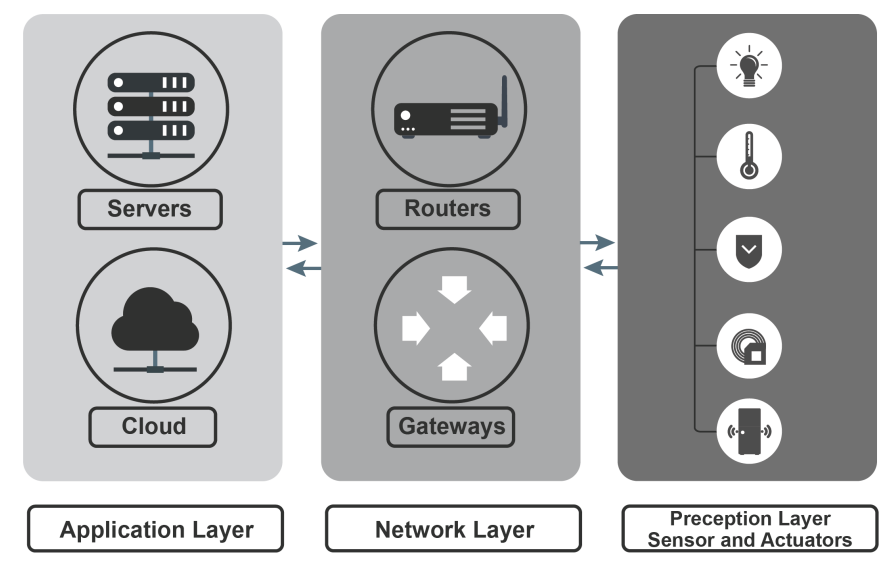
\includegraphics[width=\columnwidth]{LayersIIoT.png}
    \caption{ The three traditional IIoT Layers from \cite{SurveySecurity} }
    \label{fig1: IIoT layers }
\end{figure}
\subsection{Network Layer Attacks}
The network layer identifies a route for the message to reach receiver. It's a network of nodes that in them self could be data gathering and/or processing devices but they are also categorized in the network layer as gateways and routers. First receiver of messages from the perception layers devices communication in an network layer is called edge nodes. Not to be confused with edge computing which is a reference to all local computing power. Here follows some attacks targeting the network layer.   
\newline\newline
\textbf{Denial of Service (DoS)} attacks aim to overwhelm IIoT networks or devices with excessive traffic, making them slow or completely unresponsive. A successful DoS or Distributed Denial of Service (DDoS) attack can halt production lines, disable smart sensors or disrupt communication between critical infrastructure components. More on DDoS in later sections. 
\newline
\textbf{Sybil attacks} occur when an attacker impersonates multiple fake identities to deceive devices and disrupt communication. Making it difficult to distinguish legitimate nodes from malicious actors. Similarly, \textbf{ID Cloning Attacks} involve an attacker spoofing a legitimate device identity to gain unauthorized access and manipulate network traffic, increasing their ability to compromise connected devices. 
\newline
\textbf{Eavesdropping attacks} seems as the most obvious and gathers critics of RF-communication. Listen on the communication trying to find out as much information as possible. The message exchange can include sensitive information such as passwords and bank information in plaintext if encryption is not applied. 
\begin{figure}
    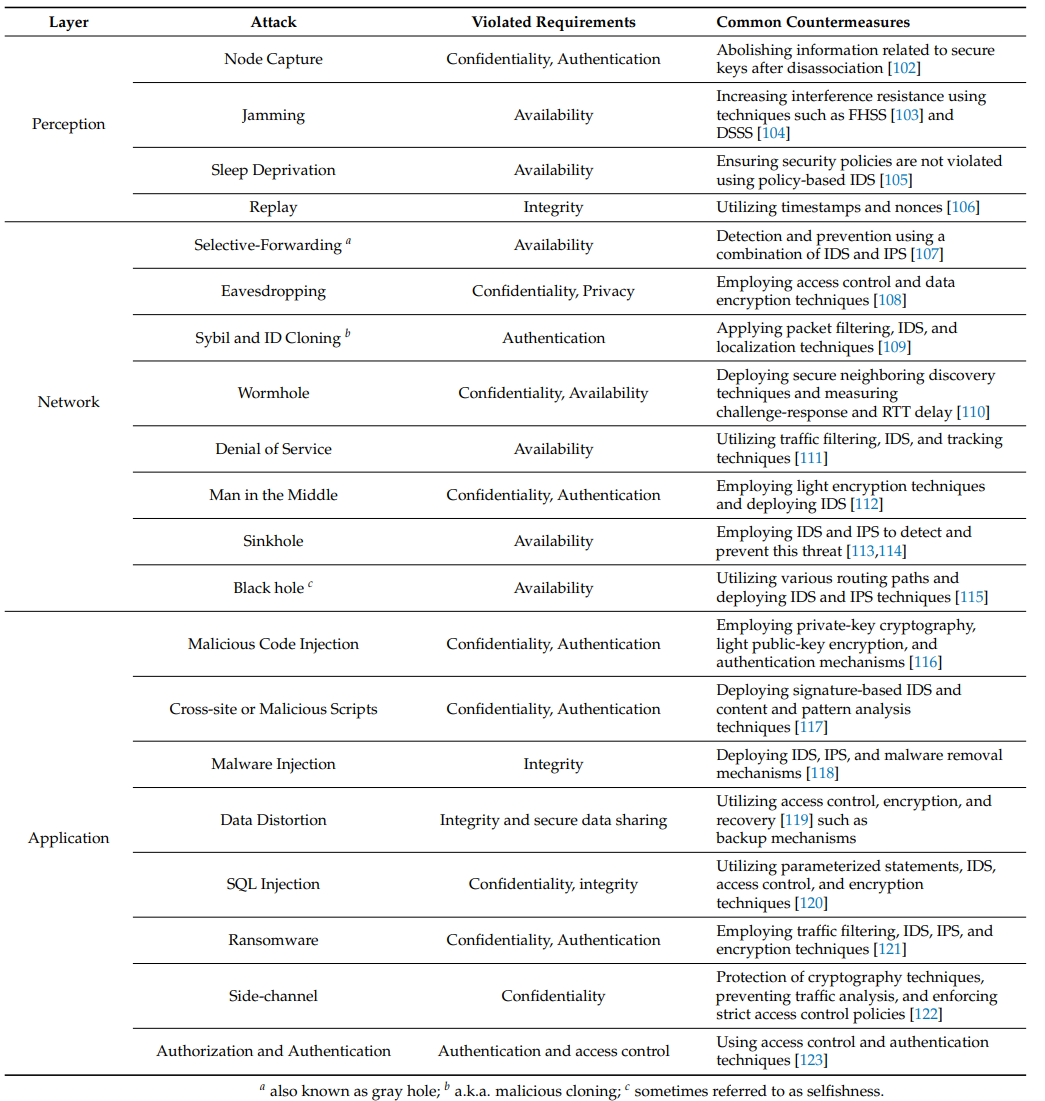
\includegraphics[width=\columnwidth]{Attackcategori.png}
    \caption{ Different attack categories table from \cite{SurveySecurity} }
    \label{fig2: Attackcategories }
\end{figure}
\subsection{Application Layer Attacks}
The application layer presents data and provides IIoT users with various applications for the manufacturing workstation. Often they are critical for the manufacturing and if no downtime is within budget for security firmware upgrades these devices that may be attached to manufacturing lines may have old firmware making them excellent targets for attackers.
\newline\newline   
Malicious software \textbf{(malware)} can infiltrate IIoT networks through infected devices, phishing emails or compromised software updates. \textbf{Ransomware} is particularly devastating as attackers encrypt IIoT data and demand payment for decryption keys, threatening manufacturing plants, energy grids and transportation system. Victims are also often willing to pay as downtime in operation could come with huge costs \cite{SurveySecurity}, making the attack worth the hackers struggle.  
\newline
IIoT devices depend on firmware updates however attackers can via \textbf{code injection attacks} infect devices during installation of updates. To protect against these attacks authentication mechanisms needs to be implemented to ensure updates installed on IIoT devices are trustworthy. 
\newline
In a \textbf{malware injection attack}, the intruder inject malware into edge devices during their service requests. Both edge servers and devices are susceptible, edge servers can be targeted by XML-, Cross-Site Request Forgery, Cross-site Scripting and Server-Side Request Forgery-injection. Edge devices are commonly attacked by Device-Side injection, commonly known as Reaper \cite{SurveySecurity}.
\newline 
In \textbf{SQL injections attacks} vulnerabilities of applications that retrieve and transmit information from and to the database is exploited. Through this kind of attacks the attacker can gain access to huge amounts of data and alter databases data and structure. 
\newline
Using \textbf{dictionary attack} the attacker use a file of the most-used passwords and tries every possible password in minutes, to determine the correct credentials that allow the attacker to gain access to the resources of a specific user or a specific device. Then in authentication and authorization attacks the attacker exploits vulnerabilities in these to reveal the authenticated username and passwords and so getting access to resources as a authorized user.
\newline\newline
IIoT systems must implement multi-layered security strategies to combat these cyber threats. By intrusion detection systems, strong encryption, policies and regular security assessments, industries can manage to mitigate these attack risks.

\section{Essential Security Requirements for IIoT Protection}
Without proper safeguards, IIoT environments remain vulnerable to cyber threats, leading to operational disruption, data breaches and financial losses. Risks that manufacturing plants are not eager to take, leading to not investing into Industry 4.0. This section outlines key security requirements necessary to protect IIoT ecosystems.
\newline 
\begin{enumerate}
    \item Authentication and Access control to prevent unauthorized access. Secure identity verification ensures that only trusted personal and devices can interact with IIoT systems. 
    \item Encryption securing data transmission between IIoT devices, cloud platforms and edge computing nodes using protocols such as TLS and AES. Encryption partly protects data from interception, manipulation and/or unauthorized alterations. 
    \item Systems implemented for threat detection and anomaly monitoring that continuously analyze network activity to identify deviations that may indicate an ongoing attack. The usage of machine learning algorithms in this key area is something discussed further.  
    \item Secure firmware and regular updates to address vulnerabilities. Legacy systems and outdated software pose significant risks, Making it essential to integrate automated authenticated update mechanisms. 
    \item Implementation of security policies where users are continuously verified and trained, reducing risk of attacks. 
\end{enumerate}

\section{The Role of AI in Industrial IoT Cybersecurity}
As IIoT networks continue to expand and cybersecurity threats comes up with new sophisticated way of intruding, machine learning will play a crucial role in detecting, preventing and mitigating attacks in IIoT environment. As stated in \cite{Deeplearning}, leveraging big data analytics and deep learning techniques to analyze network behavior and identity irregular activity helps industries respond to security threats before they escalate. 
\newline\newline
IoT botnets pose one of the threats to IIoT security, enabling large-scale cyberattacks such as DDoS attacks with remote control over compromised devices. Attackers build botnets by exploiting unprotected or misconfigured IIoT devices, turning them into a network of malicious nodes that execute coordinated attacks. In \cite{botnets} it is explored how machine and deep-learning techniques can effectively identify, predict and neutralize these threats before they cause damage. 
\newline\newline
AI-based security frameworks analyze network traffic, device behavior and communication patterns to detect anomalies linked to botnet activities. Machine learning models trained on historical attack data can recognize unusual spikes in traffic. Deep learning algorithms further enhance botnet detection by learning to distinguish normal IIoT activity from potentially compromised device behaviors, making these systems highly adaptable to new botnet variants. 
\newline\newline
One example \cite{Mirai} of how devastating IoT botnet could become was Mirai, which first emerged in 2016. Mirai targeted vulnerable IoT devices, such as IP-cameras and routers by exploiting default login credentials to gain control over them. Once infected, these devices were recruited into a massive botnet capable of executing DDoS attacks. The Mirai botnet infamously took down major websites, including Twitter, Netflix and Spotify, by overwhelming them with traffic, rendering them inaccessible. As number of IoT devices within IIoT increases a local botnet could be created by an intruder executing DDoS attacks against other critical systems in the local factory plant. 
\newline
AI-driven defense mechanism can counter similar botnet threats by employing improved threat detection, anomaly recognition, botnet identification and real-time response, strengthening industrial security. 

\section{Leveraging Edge Computing for Enhanced Security}
Edge or Fog computing place a crucial role in IIoT security by processing data closer to the source, reducing latency and minimizing exposure to external threats. By decentralizing data analysis, edge computing strengthens cybersecurity defenses although is raises new overhead for maintenance personal. It might mandate special training to more network administrators that belong to the organization making edge computing more expensive than cloud, which can be maintained by experts on the service providers side.
\newline\newline 
Bandar Alotaibis survey \cite{SurveySecurity} highlights that edge computing enables real-time security monitoring by allowing devices to detect and respond to attacks locally, minimizing the window of opportunities for intruders. Implementing intrusion detection systems (IDS), edge computing allows machine and deep-learning security models to operate directly within the networks ensuring rapid identification of malicious activity while reducing the reliance on cloud-based security solutions. 
\newline
Also having more data processed locally reduces the risk of data interception during transmission. Edge nodes can implement stronger encryption, ensuring data remains protected before being transmitted to cloud-based systems for storage and further analytics. And vise versa, firmware updates of perception layer devices can be further validated by edge nodes using cryptographic hashing and digital signatures to confirm that updates originate from trusted sources, preventing malware injection attacks. 
\section{ Case Study: The Triton Malware Attack}
The Triton malware, also known as Trisis or Hatman, was discovered in 2017 when it targeted Safety Instrument Systems (SIS) at a petrochemical facility in Saudi Arabia \cite{Triton,Triton2}. SIS are critical instruments designed to prevent hazardous failures in industrial environments, making Triton particularly dangerous. The attack gained remote access to the local network and attempted to manipulate safety controllers but was detected after an accidental shutdown, prompting an investigation that revealed the presence of the malicious Triton code embedded within the SIS controllers. 
\newline\newline
The hackers appear to have been inside the corporate network since 2014 and from there the eventually into the petrochemical plants local network. Then then got into an engineering workstation probably through flaws in operating system code or intercepting an employees login credentials. Since the workstation was communicating with plants SIS, the hackers were able to learn versions of it's system find an unknown bug in the system letting them inject code into memory that ensured they could get access to the controllers. 
\newline\newline
This attack shows that outdated firmware can contain vulnerabilities and if critical IIoT devices are not properly isolated, attackers can move laterally from compromised IoT endpoints to critical safety systems, as seen in the Triton attack. 
\section{       Conclusion}
As already discussed technologies such as machine and deep learning is going to take more space in security to detect and acting on threats. Also blockchain technology is emerging as an solution for authentication within networks. First made famous by Bitcoin, decentralizing digital currency but able to be used in other fields. This article has explored some security threats, ranging from botnet attacks and ransomware to identity cloning and unauthorized access, highlighting the vulnerabilities that IIoT networks face. 
\newline\newline
To combat these threats, industries have to look into authentication, access control, encryption, training of human staff, threat detection systems. First then investigate adopting AI-driven security solutions, which enhance threat detection, predictive monitoring and futuristic automatic defense. Additionally, edge computing plays a vital role in reducing latency while strengthening security, ensuring faster protection against attacks. 
\newline\newline
Hopefully this article has helped the reader understand some of the threats existing for current IoT and that implementing multi-layered security and continuously evolving defense capabilities is a must to keep IIoT secure and resilient so that future investments into industry 4.0 is dared by management.  
\printbibliography

\end{document}